\chapter{贪心法}


\section{Jump Game} %%%%%%%%%%%%%%%%%%%%%%%%%%%%%%
\label{sec:jump-game}


\subsubsection{描述}
Given an array of non-negative integers, you are initially positioned at the first index of the array.

Each element in the array represents your maximum jump length at that position.

Determine if you are able to reach the last index.

For example:

\code{A = [2,3,1,1,4]}, return true.

\code{A = [3,2,1,0,4]}, return false.


\subsubsection{分析}
由于每层最多可以跳\fn{A[i]}步,也可以跳0或1步,因此如果能到达最高层,则说明每一层都可以到达。有了这个条件,说明可以用贪心法。

思路一:正向,从0出发,一层一层网上跳,看最后能不能超过最高层,能超过,说明能到达,否则不能到达。

思路二:逆向,从最高层下楼梯,一层一层下降,看最后能不能下降到第0层。

思路三:如果不敢用贪心,可以用动规,设状态为\fn{f[i]},表示从第0层出发,走到\fn{A[i]}时剩余的最大步数,则状态转移方程为:
$$
f[i] = max(f[i-1], A[i-1])-1, i > 0
$$


\subsubsection{代码1}
\begin{Code}
// LeetCode, Jump Game
// 思路1,时间复杂度O(n),空间复杂度O(1)
class Solution {
public:
    bool canJump(const vector<int>& nums) {
        int reach = 1; // 最右能跳到哪里
        for (int i = 0; i < reach && reach < nums.size(); ++i)
            reach = max(reach,  i + 1 + nums[i]);
        return reach >= nums.size();
    }
};
\end{Code}


\subsubsection{代码2}
\begin{Code}
// LeetCode, Jump Game
// 思路2,时间复杂度O(n),空间复杂度O(1)
class Solution {
public:
    bool canJump (const vector<int>& nums) {
        if (nums.empty()) return true;
        // 逆向下楼梯,最左能下降到第几层
        int left_most = nums.size() - 1;

        for (int i = nums.size() - 2; i >= 0; --i)
            if (i + nums[i] >= left_most)
                left_most = i;

        return left_most == 0;
    }
};
\end{Code}


\subsubsection{代码3}
\begin{Code}
// LeetCode, Jump Game
// 思路三,动规,时间复杂度O(n),空间复杂度O(n)
class Solution {
public:
    bool canJump(const vector<int>& nums) {
        vector<int> f(nums.size(), 0);
        f[0] = 0;
        for (int i = 1; i < nums.size(); i++) {
            f[i] = max(f[i - 1], nums[i - 1]) - 1;
            if (f[i] < 0) return false;;
        }
        return f[nums.size() - 1] >= 0;
    }
};
\end{Code}


\subsubsection{相关题目}
\begindot
\item Jump Game II ,见 \S \ref{sec:jump-game-ii}
\myenddot


\section{Jump Game II} %%%%%%%%%%%%%%%%%%%%%%%%%%%%%%
\label{sec:jump-game-ii}


\subsubsection{描述}
Given an array of non-negative integers, you are initially positioned at the first index of the array.

Each element in the array represents your maximum jump length at that position.

Your goal is to reach the last index in the minimum number of jumps.

For example:
Given array \code{A = [2,3,1,1,4]}

The minimum number of jumps to reach the last index is 2. (Jump 1 step from index 0 to 1, then 3 steps to the last index.)


\subsubsection{分析}
贪心法。


\subsubsection{代码1}
\begin{Code}
// LeetCode, Jump Game II
// 时间复杂度O(n),空间复杂度O(1)
class Solution {
public:
    int jump(const vector<int>& nums) {
        int step = 0; // 最小步数
        int left = 0;
        int right = 0;  // [left, right]是当前能覆盖的区间
        if (nums.size() == 1) return 0;

        while (left <= right) { // 尝试从每一层跳最远
            ++step;
            const int old_right = right;
            for (int i = left; i <= old_right; ++i) {
                int new_right = i + nums[i];
                if (new_right >= nums.size() - 1) return step;

                if (new_right > right) right = new_right;
            }
            left = old_right + 1;
        }
        return 0;
    }
};
\end{Code}


\subsubsection{代码2}
\begin{Code}
// LeetCode, Jump Game II
// 时间复杂度O(n),空间复杂度O(1)
class Solution {
public:
    int jump(const vector<int>& nums) {
        int result = 0;
        // the maximum distance that has been reached
        int last = 0;
        // the maximum distance that can be reached by using "ret+1" steps
        int cur = 0;
        for (int i = 0; i < nums.size(); ++i) {
            if (i > last) {
                last = cur;
                ++result;
            }
            cur = max(cur, i + nums[i]);
        }

        return result;
    }
};
\end{Code}


\subsubsection{相关题目}
\begindot
\item Jump Game ,见 \S \ref{sec:jump-game}
\myenddot


\section{Best Time to Buy and Sell Stock} %%%%%%%%%%%%%%%%%%%%%%%%%%%%%%
\label{sec:best-time-to-buy-and-sell-stock}


\subsubsection{描述}
Say you have an array for which the i-th element is the price of a given stock on day i.

If you were only permitted to complete at    most one transaction (ie, buy one and sell one share of the stock), design an algorithm to find the maximum profit.


\subsubsection{分析}
贪心法,分别找到价格最低和最高的一天,低进高出,注意最低的一天要在最高的一天之前。

把原始价格序列变成差分序列,本题也可以做是最大$m$子段和,$m=1$。

\subsubsection{代码}
\begin{Code}
// LeetCode, Best Time to Buy and Sell Stock
// 时间复杂度O(n),空间复杂度O(1)
class Solution {
public:
    int maxProfit(vector<int> &prices) {
        if (prices.size() < 2) return 0;
        int profit = 0;  // 差价,也就是利润
        int cur_min = prices[0]; // 当前最小

        for (int i = 1; i < prices.size(); i++) {
            profit = max(profit, prices[i] - cur_min);
            cur_min = min(cur_min, prices[i]);
        }
        return profit;
    }
};
\end{Code}


\subsubsection{相关题目}
\begindot
\item Best Time to Buy and Sell Stock II,见 \S \ref{sec:best-time-to-buy-and-sell-stock-ii}
\item Best Time to Buy and Sell Stock III,见 \S \ref{sec:best-time-to-buy-and-sell-stock-iii}
\myenddot


\section{Best Time to Buy and Sell Stock II} %%%%%%%%%%%%%%%%%%%%%%%%%%%%%%
\label{sec:best-time-to-buy-and-sell-stock-ii}


\subsubsection{描述}
Say you have an array for which the i-th element is the price of a given stock on day i.

Design an algorithm to find the maximum profit. You may complete as many transactions as you like (ie, buy one and sell one share of the stock multiple times). However, you may not engage in multiple transactions at the same time (ie, you must sell the stock before you buy again).


\subsubsection{分析}
贪心法,低进高出,把所有正的价格差价相加起来。

把原始价格序列变成差分序列,本题也可以做是最大$m$子段和,$m=$数组长度。

\subsubsection{代码}
\begin{Code}
// LeetCode, Best Time to Buy and Sell Stock II
// 时间复杂度O(n),空间复杂度O(1)
class Solution {
public:
    int maxProfit(vector<int> &prices) {
        int sum = 0;
        for (int i = 1; i < prices.size(); i++) {
            int diff = prices[i] - prices[i - 1];
            if (diff > 0) sum += diff;
        }
        return sum;
    }
};
\end{Code}


\subsubsection{相关题目}
\begindot
\item Best Time to Buy and Sell Stock,见 \S \ref{sec:best-time-to-buy-and-sell-stock}
\item Best Time to Buy and Sell Stock III,见 \S \ref{sec:best-time-to-buy-and-sell-stock-iii}
\myenddot


\section{Longest Substring Without Repeating Characters} %%%%%%%%%%%%%%%%%%%%%%%%%%%%%%
\label{sec:longest-substring-without-repeating-characters}


\subsubsection{描述}
Given a string, find the length of the longest substring without repeating characters. For example, the longest substring without repeating letters for \code{"abcabcbb"} is \code{"abc"}, which the length is 3. For \code{"bbbbb"} the longest substring is \code{"b"}, with the length of 1.


\subsubsection{分析}
假设子串里含有重复字符,则父串一定含有重复字符,单个子问题就可以决定父问题,因此可以用贪心法。跟动规不同,动规里,单个子问题只能影响父问题,不足以决定父问题。

从左往右扫描,当遇到重复字母时,以上一个重复字母的\fn{index+1},作为新的搜索起始位置,直到最后一个字母,复杂度是$O(n)$。如图~\ref{fig:longest-substring-without-repeating-characters}所示。

\begin{center}
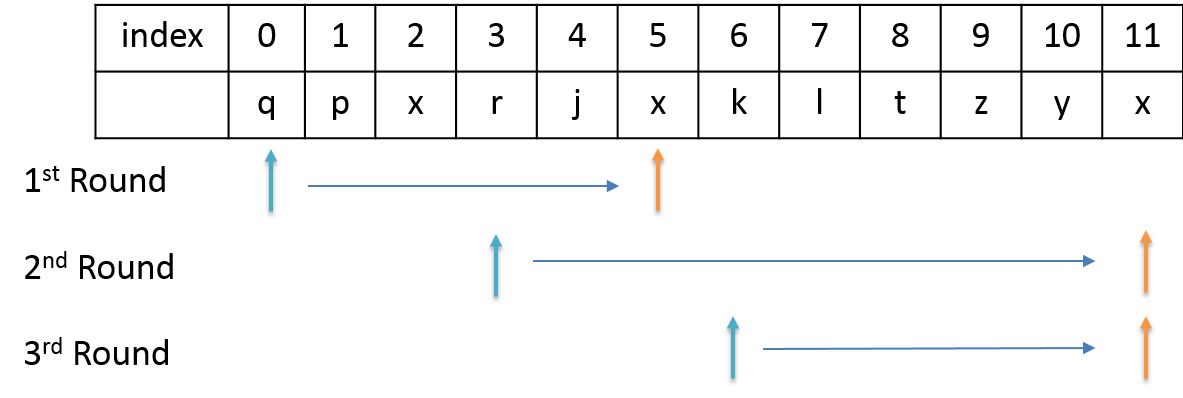
\includegraphics[width=300pt]{longest-substring-without-repeating-characters.png}\\
\figcaption{不含重复字符的最长子串}\label{fig:longest-substring-without-repeating-characters}
\end{center}


\subsubsection{代码}
\begin{Code}
// LeetCode, Longest Substring Without Repeating Characters
// 时间复杂度O(n),空间复杂度O(1)
// 考虑非字母的情况
class Solution {
public:
    int lengthOfLongestSubstring(string s) {
        const int ASCII_MAX = 255;
        int last[ASCII_MAX]; // 记录字符上次出现过的位置
        int start = 0; // 记录当前子串的起始位置

        fill(last, last + ASCII_MAX, -1); // 0也是有效位置,因此初始化为-1
        int max_len = 0;
        for (int i = 0; i < s.size(); i++) {
            if (last[s[i]] >= start) {
                max_len = max(i - start, max_len);
                start = last[s[i]] + 1;
            }
            last[s[i]] = i;
        }
        return max((int)s.size() - start, max_len);  // 别忘了最后一次,例如"abcd"
    }
};
\end{Code}


\subsubsection{相关题目}
\begindot
\item 无
\myenddot


\section{Container With Most Water}
\label{sec:container-with-most-water}


\subsubsection{描述}
Given $n$ non-negative integers $a_1, a_2, ..., a_n$, where each represents a point at coordinate $(i, a_i)$. n vertical lines are drawn such that the two endpoints of line $i$ is at $(i, a_i)$ and $(i, 0)$. Find two lines, which together with x-axis forms a container, such that the container contains the most water.

Note: You may not slant the container.


\subsubsection{分析}
每个容器的面积,取决于最短的木板。


\subsubsection{代码}
\begin{Code}
// LeetCode, Container With Most Water
// 时间复杂度O(n),空间复杂度O(1)
class Solution {
public:
    int maxArea(vector<int> &height) {
        int start = 0;
        int end = height.size() - 1;
        int result = INT_MIN;
        while (start < end) {
            int area = min(height[end], height[start]) * (end - start);
            result = max(result, area);
            if (height[start] <= height[end]) {
                start++;
            } else {
                end--;
            }
        }
        return result;
    }
};
\end{Code}


\subsubsection{相关题目}
\begindot
\item Trapping Rain Water, 见 \S \ref{sec:trapping-rain-water}
\item Largest Rectangle in Histogram, 见 \S \ref{sec:largest-rectangle-in-histogram}
\myenddot
